%! Author = erick-hdz
%! Date = 15/05/20

% Preamble
\documentclass[10pt]{report}


% Packages
\usepackage{blindtext}
\usepackage{amsmath}
\usepackage[utf8]{inputenc}
\usepackage[spanish]{babel}
\usepackage{fancyhdr}
\usepackage{graphicx}
\usepackage{algorithm, algorithmic}
\usepackage{amsfonts}
\usepackage{amsbsy}
\usepackage{makeidx}
\usepackage{geometry}
\usepackage{listings}
\usepackage[T1]{fontenc}
\usepackage{natbib}
\usepackage{amsthm}
\usepackage{amssymb}
\usepackage{lastpage}
\usepackage{multicol}
\usepackage{xcolor}

%Status of the document

\pagenumbering{roman}
\newtheorem{example}{Example}
\newtheorem{corrollary}{Corrollary}
\newtheorem*{remark}{Remark}
\newtheorem{definition}{Definition}
\newtheorem{theorem}{Theorem}
\pagestyle{fancy}
\fancyhf{}
\rhead{Sección de tesis}
\lhead{Simulación de modelos}
\rfoot{Page  \thepage}
\author{Erick Hernandez Navarrete}
\title{Simulación de modelos}


% Document
\begin{document}
    %todo:Correcciones del documento en forma de check speller
    %todo:Hacer antes de esta semana lo antes posible
    %todo:puntear a manera de commit los elementos del Cap 1
    \maketitle
    \tableofcontents{}
    \chapter{Decidibilidad en los modelos}\label{ch:decidibilidad-en-los-modelos}
    \section{Introducción}\label{sec:introducción}
    En este documento expondremos las nociones de decibilidad
    en el mundo de maquinas de Turing y en el mundo distribuido,
    asi como formalizaremos la noción de simulación de modelos
    computacionales, demostrando que el modelo $A$ de  la maquina de
    Turing es equivalente en poder al modelo distribuido $B$ en particular al modelo \textbf{LOCAL}

    \section{Decidibilidad en el modelo de maquinas de Turing}\label{sec:decidibilidasd-en-el-modelo-de-maquinas-de-turing}
    \subsection{Elementos del modelo}\label{subsec:elementos-del-modelo-de-maquina-de-turing}
    Primero enunciaremos los elementos del modelo de maquina de Turing,
    \begin{definition}%!Here we need to rewrite for errors
        Una maquina de Turing is una 7-tupla, $(Q,\sigma,\lambda,\delta,q_{0},q_{accept},q_{reject})$
        donde $Q,\sigma,\lambda$ son conjuntos finitos.
        \begin{enumerate}
            \item $Q$ es el conjunto de estados,
            \item $\Sigma$ es el alfabeto de entrada que no contiene el simbolo blanco $\sqcup$
            \item $\Lambda$ es el alfabeto de la cinta, donde  $\sqcup\in\lambda$ y ademas $\lambda$,
            \item $\delta: Q\times\Omega \rightarrow Q\times\Omega\times\{L,R,S\}$ es la función de transición,
            \item $q_{0}$ es el estado de iniciación,
            \item $q_{accept}$ es el estado de aceptacion
            \item $q_{reject}$ es el estado de rechazo,donde $q_{accept} \neq q_{reject}$,

        \end{enumerate}

    \end{definition}
    Esta definición esta encapsulando los elementos del modelo,
    asi que una vez que tenemos los elementos, podremos definir la semantica
    de que un problema se soluble en este clasico modelo,definiendo
    la noción de decidibilidad.
    \space
    %!Final de las observaciones de la edicion de este capitulo.
    \subsection{Decidibilidad}\label{subsec:decidibilidad2}
    Podemos observar que este modelo, las estructuras de datos que están consumiendo
    son cadenas a priori finitas, entonces una vez que le damos como entrada a una maquina de
    Turing una cadena $w$, podemos decir que esa cadena es aceptada o rechazada,
    entonces definimos lo siguiente:
    %!Aqui vamos a definir antes que nada los elementos que consitituyen la aceptación

    \begin{definition}
        Sean $x,y$ dos cadenas, y $q_{j}$ con $j\in I$, un estado en el conjunto de estados $Q$,
        estos elementos del modelo Turing conformaran una semántica:
        $xq_{j}y$ donde la posición del estado representa la localidad del
        cabezal en ese momento del computo.
        Para esa triada $x,q_{j},y$ definira la noción de configuración,
        que la denotaremos de la siguiente manera $C_{j}$.
    \end{definition}

    Una vez que tenemos la definición formal de \textbf{Configuración},
    nos movemos a conectar esta idea con la noción de computo.
    \begin{definition}
        Sean $C_{1}, C_{2}$ configuraciones:\newline
        vamos a decir que $C_{1}$ produce a $C_{2}$  legalmente en un solo paso si semánticamente pasa
        lo siguiente:
        Sea $a,b y c \in \Omega$ y tomamos también $u,v$ cadenas y tenemos el
        siguiente contexto:
        $uaq_{i}bv$ produce $uq_{j}acv$ si $\delta(q_{i},b) = (q_{j},c,L)$
        donde $R,L,S$ son para denotar la semantica del movimiento del cabezal,
        derecha, izquierda o en su defecto no moverse.\newline
        En el caso de un movimiento a la derecha es:
        $uaq_{i}bv$ produce $uacq_{j}v$ si $\delta(q_{i},b) = (q_{j},c,R)$.

    \end{definition}
    \newline
    La definición anterior formalizara  la noción de la secuencias  de configuraciones, que en esencia
    esta formalizando la noción de computo.
    \space
    \begin{definition}
        Decimos que tenemos una configuración inicial para $M$ una máquina de Turing y $w$ con
        entrada una cadena $w$ a la configuración: $C_{0}$ escrita de la siguinte manera:
        $q_{0}w$.
        El cual indica que la máquina esta en su estado inicial $q_{0}$ con su cabezal en el última
        localidad del lado izquierdo.
    \end{definition}
    \begin{definition}
        \newline
        \begin{itemize}
            \item En una configuración de aceptación tenemos el estado $q_{accept}$
            \item En una configuración de rechazo tenemos el estado $q_{reject}$.
        \end{itemize}
    \end{definition}
    %!Aqui estamos haciendo enfasis de que en estas tesis.
    %!Los hechos
    \begin{remark}
        Podemos clasificar a las configuracione de la siguiente manera:
        \begin{itemize}
            \item  Configuraciones de detención
            \item Y las que no son.
        \end{itemize}
        Dichas configuraciones tienen la propiedad de no producir otra configuración $C_{k}$,
        en otras palabras son configuraciones finales.
        Las configuraciones que son de dicha naturelaza, son la configuración de \textbf{aceptacioń}
        y la configuración de \textbf{rechazo}.\newline
        Mas aún podriamos complicar la función $\delta$
        tomando $Q^* = Q-\{q_{accept}, q_{reject} \}$\newline
        y redefinimos a delta como:\newline
        $\delta:Q^*\times\Omega\leftarrow Q\times\Omega\times\{L,R,S \}$
    \end{remark}
    %!Podemos dificultar un poco mas la notación de la funcion \delta, perforando en la entrada estados
    %!Estados de paro, tal y como lo podemos ver.

    \theoremstyle{definition}
    \begin{definition}
        Decimos que una máquina de Turing \textbf{acepta} una entrada $w$ si existe una secuencia de configuraciones
        $C_{1},\mathellipsis,C_{k}$ tal que:
        \begin{enumerate}
            \item $C_{1}$ es la configuración inicial
            \item Cada $C_{i}$  produce $C_{i+1}$ y
            \item $C_{k}$ es la configuración de \textbf{aceptación}.
        \end{enumerate}
    \end{definition}

    \theoremstyle{definition}
    \begin{definition}
        Sea M una máquina de Turing.
        La colección de cadenas tales que $M$ las acepta,
        es un \textbf{lenguaje} que acepta ó que es reconocible por $M$, y lo denotamos
        de la siguiente manera: $L(M)$.
    \end{definition}
    Mas aun podemos definir la siguiente nocion:
    \begin{definition}
        Llamamos a un lenguaje \textbf{Turing-Reconocible} si existe una
        máquina de Turing que lo reconozca.
    \end{definition}
    \begin{remark}
        Cuando iniciamos una máquina de Turing con entrada $w$, pueden pasar tres escenarios:\newline
        \begin{itemize}
            \item acepta,
            \item rechaza,
            \item nunca se detiene.
        \end{itemize}
    \end{remark}
    %!Aqui vamos a hacer el enfasis de que siempre tendremos maquinas que paren.
    En este caso, tomaremos solamente máquinas de Turing que se detienen para todas sus entradas,
    por lo tanto dichas máquinas siempre se dentendrán en algún momento de la
    ejecución de $M$ para $\forall w$ entrada.
    Formalizaremos lo anterior con una definición:
    \space
    \begin{definition}
        Sea $M$ máquina de Turing tal que $\foraall w$ entrada se detiene en algún momento de la ejecución,
        entonces decimos que dicha máquina de Turing tiene el atributo de ser
        \textbf{decidible}\newline
        Es decir, siempre entrán en su estado de \textbf{aceptación}
        o en su estado de \textbf{rechazo} en algún momento de la ejecución.
    \end{definition}
    Y por el lado de la noción del lenguaje definimos lo siguiente:
    \begin{definition}
        Decimos que un lenguaje es \textbf{decidible} si existe un máquina de Turing
        que lo \textbf{decide}.
    \end{definition}
    %!Exponer un ejemplo de máquina de Turing, tanto en esta version, como en la versión final de esta tesis
    \subsubsection{Ejemplo de lenguajes decidibles}
    A continuación describiremos un ejemplo de una máquina de Turing, describiendo cáda una de sus partes que la definen,
    así como el principio de funcionamiento de la misma.
    \begin{example}
        Tomamos el siguiente lenguaje:
        \begin{equation}
            A = \{ 0^2^n : n>=0\}\label{eq:equation2}
        \end{equation}
        Es el lenguaje que consta de cadenas de 0's tal que su longitud es una
        potencia de 2.
    \end{example}
    Entonces afirmamos que $M_{2}$ es un lenguaje decidible.
    %!Hacer un sketch de que es un lenguaje decidible
    Entonces podemos hacer las instrucciones (alto  nivel) para $M_{2}$ como sigue:
    \begin{enumerate}
        \item recorrer de izquierda a derecha a través de la cinta, tachando uno de cada dos ceros.
        \item Si en la etapa 1, la cinta contenia un solo $0$,entonces \textbf{acepta}.
        \item Si en la etapa 1, la cinta contenía mas de un $0$ y ademas contenía un numero impar, mayor a $1$, \textbf{rechaza}.
        \item Regresa el cabezal al lado izquierdo al final de la cinta.
        \item Ve a la etapa 1.
    \end{enumerate}
    Una vez que tenemos la descripción de la máquina de Turing a un alto nivel, podemos hacer un puente
    a un bajo nivel, que es formalmente describir la máquina con sus elementos que la definen para una entrada $w$,
    el cual nuestro puente será en describir la función $\delta$ vía un diagrama de estados.


    %!Describiendo el alto nivel de la maquina de Turing a un alto nivel.
    En la etapa 1 de $M_{2}$ corta el número de ceros a la mitad.Mientras la máquina barre a tráves de la cinta en la
    etapa 1, lleva la cuenta de $0$'s vistos si es par o impar. Si el número es impar mayor a 1,entonces el número original
    de $0$'s en la entrada no puede ser una potencia de 2. Entonces la máquina \textbf{rechaza} en esa instancia.
    Como sea, si el número de 0's visto es 1, entonces el número original tiene que ser una potencia de 2, entonces en ese
    caso la máquina \textbf{acepta}.
    %!Descripción formal de la máquina de Turing.
    Sea $M_{2} =(Q,\Sigma,\Lambda,\delta,q_{1},q_{accept},q_{reject})$:
    \begin{enumerate}
        \item $Q = \{q_{1},q_{2},\dots,q_{5},q_{accept},q_{reject}$,
        \item $\Sigma = \{ 0 \}$ and
        \item $\Lambda = \{0,x,\sqcup \}$.
        \item Describirimos a $\delta$ con un diagrama de estado.
        \item Los estados de inicio, aceptación y rechazo son $q_{1},q_{accept},q_{reject}$ respectivamente.
    \end{enumerate}
    \newline
    \begin{center}
        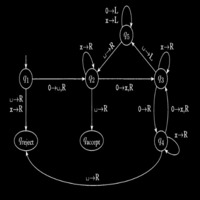
\includegraphics{Im_1.jpg}
    \end{center}
    \newline
    En este diagrama, la etiqueta $0\rightarrow \sqcup,R$ que aparecé en la transición del estado $q_{1}$ al estado $q_{2}$,
    tiene la semántica de la definición de la función $\delta$, que en otras palabras se describe como si:
    en el estado $q_{1}$ con el cabezal leyendo $0$, la máquina va al estado $q_{2}$, escribe $\sqcup$ y mueve el cabezal
    a la derecha.\newline
    Lo cúal en términos formales significa que: $\delta(q_{1},0) = (q_{2},\sqcup, R)$.
    Otra escritura que usaremos para hacer la notación en este ejemplo mas compacta,
    es denotar: $0\leftarrow R$, que la semántica es que se hace la transición del estado $q_{3}$ al estado $q_{4}$, que
    es la etiqueta que se aprecia en el diagrama de estados, y ademas significa que la máquina se mueve a la derecha en
    el momento en el que lee un $0$ en el estado $q_{3}$, pero que no altera la cinta(\no hace una operación escritura),
    entonces $\delta(q_{3}),0) = (q_{4},0,R)$ en términos del mapeo que se esta generando.
    Esta máquina inicia escribiendo un simbolo blanco sobre el ulti|mo $0$ de lado izquierdo. En particular esto sirve
    para delimitar el final de la cinta con el simbolo blanco $\sqcup$ en esta particular máquina de Turing.
    \space
    Ahora vamos a hacer una ejecución de Turing para la entrada $w = 0000$, en el cual escribiremos la función
    transición $\delta$ con la semántica de las configuraciones.
    
    %!Here we can use the next sessions of the rows as we can see
    La siguiente secuencia es la ejecución de $M_{2}$ con la entrada en particular $w = 0000$,
    Se lee hacía abajo de las columnas de izquierda a derecha.

    \begin{center}
        \begin{tabular}{c c c}
            $q_{1}0000$ &     $\sqcup q_{5}x0x\sqcup$ & $\sqcup xq_{5}xx\sqcup$ \\
            $\sqcup q_{2}000$ & $q_{5}\sqcup x0x\sqcup$ & $\sqcup q_{5}xxx\sqcup$\\
            $\sqcup xq_{3}00$ & $\sqcup q_{2}x0x\sqcup$ & $q_{5}\sqcup xxx\sqcup$\\
            $\sqcup x0q_{4}0$  & $\sqcup xq_{2}0x\sqcup$ &   $\sqcup q_{2}xxx\sqcup$\\
            $\sqcup x0xq_{3}\sqcup$ & $\sqcup xxq_{3}x\sqcup$ & $\sqcup xq_{2}xx\sqcup$ \\
            $\sqcup x0q_{5}x\sqcup$ & $\sqcup xxxq_{3}\sqcup$ & $\sqcup xxq_{2}x\sqcup$ \\
            $\sqcup xq_{5}0x\sqcup$ & $\sqcup xxq_{5}x\sqcup$ & $\sqcup xxxq_{2}\sqcup$ \\
                            &                                 & $\sqcup xxx\sqcup q_{accept}$ \\
        \end{tabular}
    \end{center}


    %! Final del ejemplo de la máquina de Turing.Inicio de la teoria de Computo Distribuido.

    \section{Decidibilidad en el modelo de computo distribuido  \textbf{LOCAL}}\label{sec:decidibilidad-en-el-modelo-de-computo-distribuidotextbf}
    Ahora lo que haremos es definir el modelo de computo distribuido de manera formal,
    y tomar un modelo en particular en la que enfocaremos nuestro estudio, para posteriormente
    estudiar la noción de decibilidad en dicho modelo.

    %!Aqui las correcciones que hemos hecho son esencialmente triviales

    \subsection{Presentación del modelo de computo distribuido}\label{subsec:presentación-del-modelo-de-computo-distribuido}
    \subsubsection{Presentación del protocolo de comunicación}
    Este modelo tendrá una capa de abstracción de comunicación, asi como su respectiva capa de
    computación de la siguiente manera.
    \subsubsection{Capa de comunicación}
    El modelo de comunicación consiste en una red de comunicación 1-1 que será descrita en términos formales por
    una gráfica conexa, no dirigida $G=(V,E)$, donde los vertices $V=\{ v_{1},\mathellipsis v_{n} \}$.
    operando entre ellos.
    Inicialmente, consideraremos identificadores unicos asignados a los procesos de la gráfica $G$.\space
    Má||s concretamente consideraremos a estos identificadores de un conjunto ordenado de enteros:
    de la siguiente manera:

    \begin{equation}
        S = \{ s_{1},\mathellipsis,s_{n}\} \
        donde:\ s_{i} < s_{i+1} \ \forall i\leq 1\label{eq:equation}
    \end{equation}
    Entonces con esta notación, una ID-asignación es un mapeo:
    $ID:V\rightarrow S$ entonce nos referiremos a su identificador como:
    $ID(v)$. \newline
    Entonces la comunicación se llevara acabo de la siguiente manera: \newline
    Cada vertice tendra asociado el numero de puertos, como el $deg_{G}(v)$,
    entonces en este sentido, el conjunto de aristas adyacentes al vertice
    contiene exactamente $deg_{G}(v)$, donde cada arista esta conectado en un puerto de v.
    \newline
    Podemos denotar que a cada arista $(u,v)$ le corresponde la pareja
    $((u,i),(v,j))$ donde $1\leq i \leq deg_{G}(u) $ y $1\leq j \leq deg_{G}(v)$,
    con semántica: \textbf{un canal de comunicación conectadose en el puerto $i$  de $u$ con el puerto $j$ de
    $v$.}\newline
    El vertice $u$ envía un mensaje a sus vecinos $v$ cargando el mensaje en puerto apropiado, digamos $i$.
    Este mensaje es recivido por $v$ a tráves del puerto $j$. \newline
    %!Aqui se ha acaabado las correcciones de la capa de comunicacion.

    %!Inicio de las correcciones de la capa de computacion.
    \subsubsection{Capa de Computación}
    Una vez que tenemos la capa de comunicación, presentaremos la capa formal del modelo de
    computo.
    El modelo estara governado por un algoritmo $\Pi$ que estara compuesto de protocolos
    $\Pi_{1},\mathellipsis,\Pi_{n}$ donde cada $\Pi_{i}$ residira en el vertice $v_{i}$.
    \newline
    \begin{remark}
        Hasta ahora hemos hablado a secas de los vertices,pero podemos darle una semantica
        de computo en términos de \textbf{procesos}, el cual significa que es una entidad de computo, y entonces a cada $v_{i}$
        lo nombraremos como el proceso $p_{i}$.\newline
        Con esta convecion podemos decir que para $\Pi_{i}$ residira en su respectivo proceso:
        $p_{i}$.

    \end{remark}
    %!Aqui haremos el entendimiento computacional de los procesos.
    \begin{remark}
        Podemos observar que podemos modelar a cada $\Pi_{i}$ como una maquina de estado para $\forall i$ con su
        correspodiente conjunto de estados estado $Q_{i}$ conteniendo su estado inicial  $q_{0i}$ y sus estados de
        aceptación y rechazo: $q_{accept},q_{reject}\in Q_{i}$ respectivamente tal que en cualquier
        momento dado el proceso $p_{i}$ esta en el estado $q_{i}$ de $Q_{i}$.
        \space
        Mas aún podemos pensar en cada $\Pi_{i}$ como en una maquina de Turing con operaciones de envio y
        recepción de \textbf{mensajes}.
    \end{remark}
    %!Lo anterior nos da el preambulo de ver a cada algo como una maquina de Turing.
    \newline
    Por otro lado en la capa de comunicación tendremos el siguiente esquema:
    \newline
    %!Aqui vamos a dar una definición formal de lo que es un mensaje en un
    %!Manejador de contexto.
    \begin{definition}
        Vámos a definir un mensaje $MSG$ como la información local que sera enviada del proceso $v$ al proceso $u$,
        por medio del canal $((v,i),(u,j))$, donde el proceso $u$ tiene el atributo de la operacion $send$,\space
        para el cual cada proceso tiene un puerto de entrada por cada
        canal de comunicación adyacente, en el cual es añadida la información $MSG$, y el cual el proceso hace una operación
        de lectura para dicha entrada.
        \newline
        Podemos decir que el tamaño de la información del mensaje $MSG$, es $\O(\log n)$ bits.
    \end{definition}

    En cualquier momento dado y en cualquier canal de comunicación $e_{i}=(u,v)$ está en algun estado
    $\overline{q}_{i}$ del conjunto de estados $\overline{Q}_{i}$
    el estado $\overline{q}_{i}$ esta compuesto de dos componentes denotadas de la siguiente manera:
    $\overline{q}_{u\leftarrow v}$ y $\overline{q}_{v\leftarrow v}$ una por cada direccion del canal
    de comunicación.
    Vamos a denotar como $M$ cómo la colección  de todos los posibles mensajes que se pueden enviar de un proceso a otro en toda ejecucion del algoritmo,
    \space cada uno de los dos componentes $\overline{q}_{u \leftarrow v}$ es un elemento de $M \cup \lambda$,
    $\overline{q}_{u\leftarrow v} = MSG\in M$ significa que ahora el mensaje $MSG$ esta en transicion de
    $u$ a $v$, y denotaremos que $\overline{q}_{u\leftarrow v} = \lambda$ para representar una semantica de que
    el canal actual esta vacio en esa dirección.
    En el inicio del computo, todos los procesos estan en el estado inicial $q_{0,i}$ $\forall i$
    y todos los canales de comunicación estan vacios.
    Es decir que sintacticamente: $\overline{q}_{i,0} = <\lambda,\lambda>$
    \subsubsection{Ejecución de un algoritmo en este modelo}
    La ejecución del algoritmo en este ambiente consistira de \textbf{Eventos} ocurriendo en diversos
    lugares de la red y afectando a los procesos involucrados.
    Diremos que un \textbf{paso computacional} es una operación como máquina de Turing del proceso $p$.
    Los eventos puede ser del tipo:
    \begin{itemize}
        \item Computacional:representando un paso en un procesador
        \item Comunicación: representando la entrega o la recepción de un mensaje.
    \end{itemize}
    Donde cada evento de comunicación tiene una semántica de:
    $SEND(i,j,MSG)$ o $DELIVER(i,j,MSG)$ para algún $MSG\Mu$.
    Entonces a manera de reportorio de eventos tenemos:
    \begin{enumerate}
        \item Evento $COMPUTE(i)$:El proceso $v_{i}$ ejecuta una operación interna, basado en su estado local, y
        posiblemente cambie su estado local.
        \item Evento $SEND(i,j,MSG)$:El proceso $v_{i}$ envia de salida un mensaje $MSG$ en algún canal de
        comunicación link $e_{l}$ con destino al proceso $v_{j}$
        \item Evento :$DELIVER(i,j,MSG)$: El mensaje $MSG $ originado de un proceso $v_{i}$
        que es enviado por el canal de comunicación $e_{l}$ es entregado en la entrada del destino $v_{j}$
    \end{enumerate}
    Entonces la computación en un sistema distribuido lo podemos pensar de la siguiente manera:
    Como una secuencia de configuraciones, capturando el estado actual de los procesos y los canales de comunicación.\newline
    Cada evento cambia de estado para algun procesador $v_{i}$, y posiblemente también para un canal de comunicación
    y eso cambiara la configuracion del sistema.
    En terminos formales lo podemos pensar de la siguiente manera:
    \theoremstyle{definition}
    \begin{definition}
        Una configuracion es una tupla $(q_{1},\mathellipsis,q_{n},\overline{q}_{1},\mathellipsis,\overline{q}_{m})$
        donde $q_{i},\overline{q}_{j}$ es el estado del procesador $p_{i}$ y del canal de comunicación $e_{j}$ respectivamente
        y la configuración inicial es:
        \begin{equation}
        q_{0,1},\mathellipsis,q_{0,n},\overline{q}_{0,1},\mathellipsis \overline{q}_{0,m}\label{eq:equation5}
        \end{equation}
        \newline
        \begin{remark}
            Como estamos pensando de manera intuitiva a cada uno de los procesos como una máquina de Turing, entonces
            una vez que uno de los procesos entra en alguno de los estados:\space $\q_{accept},q_{reject}$, el proceso ya no cambía
            de estado, pero sus operaciones de envio y recepción de mensajes siguen activos.
        \end{remark}
        \newline
        Entonces modelaremos la computación del algoritmo como una (posible) infinita secuencia de configuraciones
        alternadamente con eventos.
    \end{definition}
    \theoremstyle{definition}
    \begin{definition}
        La ejecución de un algoritmo $\Pi$ en una grafica con cierta topologia
        $G$ con una entrada inicial $I$ en los procesos es denotado como $\kappa_{\Pi(G,I)}$.
        Formalmente, una \textbf{ejecución} es una secuencia de la forma:
        \begin{equation}
            \kappa = (C_{0},\rho_{1},C_{1},\rho_{2},C_{2},\mathellipsis)\label{eq:equation3}
        \end{equation}
        donde cada $C_{k}$ es una configuración y cada $\rho_{j}$ es un evento,
        y en particular $C_{0}$ denota la configuración inicial.
    \end{definition}
    %!Mejorar la explicacion del modelo LOCAL.
    Podemos imponer ciertas restricciones en las ejecuciones del algoritmo, pero por el momento
    podemos definir formalmente el concepto $\modelo$ en terminos de ejecuciónes para algun algoritmo
    $\Pi$\newline
    Entonces lo anterior nos permite definir lo siguiente:
    \begin{definition}
        Diremos que un modelo es un subconjunto de esas posibles ejecuciones
    \end{definition}
    Con la definición anterior, nos basaremos en un modelo en particular con una propiedad en particular, a saber el que
    tiene una estructura de rondas.\newline
    \begin{definition}
        Diremos que un \textbf{modelo} tiene el atributo de rondas si:
        \begin{enumerate}
            \item Cada proceso $p$ ejecuta \textbf{send} a todos sus vecinos, \textbf{deliver} de todos sus vecinos y finalmente \textbf{compute},
            \item Cada proceso ejecuta su $r$-ésima ronda si todos los procesos ejecutaron su $r-1$ ronda.
        \end{enumerate}
    \end{definition}\newline
    La definición anterior nos permitira definir el siguiente modelo:
    \begin{definition}
        Llamaremos $LOCAL$ al modelo que posea la estructura de rondas.
    \end{definition}
    Y podemos observar que el punto 2 de la definición de rondas, es lo que da el cáracter de
    síncronia en la ejecución.
    %!Aqui lo que haremos es hacer es tratar de ser lo más claro en las nociones
    %!Enunciados
    \subsubsection{Ejemplos}
    %!todo:Pegar el ejemplo del algoritmo en LOCAL para la versión final de la tesis.


    \newpage
    \subsection{Decidibilidad}\label{subsec:decidibilidad}
    Una vez que tenemos los elementos del modelo distribuido, podemos introducir la noción de \textbf{decibilidad}, en
    este modelo de computo formal.

    \theoremstyle{definition}
    \begin{definition}
        Sea $w$ una cadena, podemos escribir a la cadena como $w_{0},\mathellipsis, w_{n}$, la cual sera la entrada al algoritmo
        $\Pi(w)$, donde de manera distribuida, tendremos como inicialización, que cada proceso $p$ tendra como entrada un caracter de la cadena $w$, digamos $p_{j}(w_{k})$.\newline
        Sea $\kappa_{\Pi(w,G)}$ una ejecución del algoritmo $\Pi$ con entrada $w$ en la grafica $G$, entonces diremos que
        la entrada $w$ es aceptada, si existe una configuración en la ejecución $\kappa_{\Pi(w,G)}$, digamos $C_{k}$ tal que
        existe un estado $q_{a}$ en $C_{k}$, de su correspondiente proceso $p_{a}$, tal que $q_{a}=q_{accept}$.\newline
        Es decir, que el estado en esa configuracion es exactamente el estado $q_{accept}$.\newline
        En simbolos:
        \begin{equation}
            \forall \kappa_{\Pi(w,G)},\ \exists C_{K}\ \mid \exists p_{a}\ \mid q_{a}=q_{accept}.\label{eq:equation4}
        \end{equation}
    \end{definition}

    %!--En otras palabras lo que quiere decir es lo siguiente --!%
    Lo anterior, nos permitira definir lo siguiente:
    \begin{definition}
        Al conjunto de cadenas que acepta un algoritmo distribuido $\Pi$ es el lenguaje
        de $\Pi$, o el lenguaje que decide $\Pi$, y lo denotaremos como $L(\Pi)$.
    \end{definition}


    %todo:Migrate the chapter to another file .tex e incluirlo en un main .tex
    \chapter{Simulación de modelos Maquina de Turing y \textbf{LOCAL}}\label{ch:simulacion-de-modelostextbfytextbf}
    \section{Noción de simulación en modelos}\label{sec:nocion-de-simulación-en-modelos}
    Una vez que tenemos estos dos modelos de computo formal, a nivel logico podemos decir que:
    \theoremstyle{definition}
    \begin{definition}
        Decimos que un modelo $T$ simula un modelo $S$ si:
        \begin{equation}
        \forall x\in L(S) \ entonces \ x\in L(T)
        \end{equation}
        Mas aún decimos que son modelos equivalentes (computacionalmente) si:
        \begin{equation}
        \forall x\in L(T) \iff x\in L(S) \
        \end{equation}
    \end{definition}
    \space
    Entonces enunciaremos nuestro teorema de la siguiente manera:

    \begin{theorem}
        Sea $TM$ una maquina de Turing, entonces existe un $\Pi$ algoritmo distribuido que simula
        a $TM$,con la semántica de \textbf{simulación} con base a la definición anterior.
    \end{theorem}
    Una vez esto nos podemos adentrar en el diseño de un algoritmo en el que burdamente le daremos en la entrada una
    rebanada de la cadena que es aceptada por una maquina de Turing en Abstracto y que es aceptada por dicho algoritmo.
    %the subsection of the algorithm as we can see

    \section{Diseño del algoritmo}\label{sec:diseño-del-algoritmo}
    \begin{remark}
        Trivialmente podemos pensar que al darle la entrada la cadena que es aceptada por una maquina de Turing,
        es consumida, tal que cada proceso la tiene enteramente como entrada, i.e $\Pi(w)$ entonces de manera local se da
        que $v_{j}(w)$ entonces esta en particular que en algun momento de la ejecucion el estado de ese proceso localmente,
        $q_{i}\gets q_{accept}$ entonces $w\in L(\Pi)$, pero podemos observar que la forma de la entrada en el algoritmo $\Pi$
        es de manera no distribuida.
    \end{remark}
    Entonces no es verdaderamente un diseño de un algoritmo distribuido,por lo tanto procederemos a diseñar de manera
    distribuida el siguiente algoritmo:
    \space
    %Una vez que tenemos esta información daremos una capa de adversario tal y como lo haremos de esta manera
    %En esta parte daremos una part externa que es la noción de rival en el siguiente sentido
    Daremos la distribución de la información a manera de contricante de la siguente manera:
    Sea $w\in L(TM)$ para una maquina de Turing $TM$ arbitraria, entonces decimos que una rebanada de la cadena
    $w[i]$ tiene localidad $i$.
    Esta semantica nos va a permitir definir lo siguiente:
    \theoremstyle{definition}
    \begin{definition}
        Sea un $v_{k}$ un proceso del modelo en particular $\text{LOCAL}$ diremos que dicho proceso
        tendra como entrada a una rebanada $w_{i}$ de la cadena $w$ denotada tambien como
        $w_{j}$, de localidad $j$
    \end{definition}
    En general podremos alimentar a cada proceso con una familia de rebanadas de cierta localidad.
    Esto nos da la noción del control externo de las entradas, que por el momento esto nos esta generando
    una cierta familiaridad del papel a un alto nivel de la visión del contrincante como podremos observar
    esta es la contraparte del algoritmo que esta gobernando computacionalmente (o por la capa de computo)
    por el algoritmo.
    \space
    Entonces nos propondremos el siguiente diseño del algoritmo que nos dara a priori
    la solución del problema que estamos atacando.

    %!---Esta es el diseño sin las definiciones anteriormente enunciadas --!%
    %!---Esto por la nocion del adversario que hemos enunciado anteriormente ---!%
    \begin{algorithm}
        \caption{$Simula\char95Algo\char95TM(w)$}\label{simula}
        \begin{algorithmic}
            \STATE $w_{1}\mathellipsis w_{k} \gets w$
            \STATE \textbf{Síncronamente}
               %!--Aqui estamos mapeando cada evento del tipo Comp con cada ronda ---!%
               \FORALL{$r=1$ \TO $n$}
                  \STATE $v_{j}(w_{i})$\COMMENT{Codigo para $v_{j}$}
                  \STATE $q_{j}\gets q_{0}$\COMMENT{Poner estando inicial en 0}
                  \WHILE{\textbf{true}}
                     \STATE \textbf{call} $\delta(q_{j},w_{i})$
                     \STATE $(q_{r},w_{r},P)\gets \delta(q_{j},w_{i})$
                  \ENDWHILE
                  \IF{$q_{r}=q_{accept}$}
                     \RETURN{$q_{r}$}
                  \ELSE
                     \STATE $\textbf{send}(t,MSG\gets<q_{r},w_{r},P>)$
                  \ENDIF
               \ENDFOR
        \end{algorithmic}
    \end{algorithm}
    \space
    %!--El siguiente capitulo es la descripción del algoritmom ----!%
    \section{Descripción del algoritmo}\label{sec:descripción-del-algoritmo}
    Entonces lo que podemos observar que en esencia estamos delegando con la función $\delta$
    que es parte de la información local del proceso $v_{j}$ pero tendremos un control en el que de manera implicita
    por la parte que esta teniendo la visión del contrincante,que es la naturaleza de la distribución de la información,
    en las entradas del buffer de cada $v_{j}\in V(G)$, donde la naturaleza topologica de $G$ es abstracta a priori.
    Pero la logica del token es que esta llamada sera iterada hasta que la rebanada de la cadena que nos da la invocacioń
    de $\delta$ sea una rebanada de localidad correspondiente al actual proceso que esta teniendo el evento $COMPUTE(j)$.
    Asi cuando esto sea falso, tendra una logica de aceptación o en su defecto de iniciar un evento del tipo de
    comunicación: $SEND(j,t,MSG)$ donde el $MSG$ es lo que nos arroja el ultimo llamado de $\delta$, donde $t$, denota
    sin perdida de generalidad el indice de uno de sus vecinos.
    \space
    Asi que enunciaremos los siguientes afirmaciones a manera de teorema del cual se desprendera la simulación de $TM$
    maquina de Turing via el modelo $LOCAL$.\newpage

    \section{Demostración del procedimiento $Simula\char95Algo\char95TM$}\label{sec:demostración-del-procedimiento}
    %!--Primera parte demostrativa del teorema --%!
    \begin{theorem}
        El algoritmo $Simula\char95Algo\char95TM$ es correcto.
    \end{theorem}
    \begin{proof}
        Sea $r$ una ronda de la ejecución del algoritmo $\Pi=Simula\char95Algo\char95TM$,
        al incio de esa ronda se estara iniciando un evento del tipo $COMPUTE(k)$, de nuestro repertorio de eventos para el proceso
        $v_{k}$, por la naturaleza de la distrubución de la información llegara un momento
        de la iteración en la que  se de una estructura de dato $msg\gets <q_{r},w_{r},P>$ arrojada por el llamado iterativo de
        $\delta$, ya que la localidad de $w_{r}$ no esta asignada a $v_{k}$ sin perdida de generalidad.
        Entonces siguiendo el codigo, observamos que tenemos una logica para la estructura de dato:
        si $q_{r}=q_{accept}$ entonces $w\in L(\Pi)$ y se acabaria la ejecución en dicha ronda.
        Si no, entonces se activa el evento $Send(t,MSG)$,donde sin perdida de generalidad $t$ representa el indice de uno de los vecinos
        del proceso $k$, por otro lado como $w\in L(TM)$ entonces $\exists v_{l}$ en la ronda $r+1$
        tal que al final dicha ronda $\exists q_{l}$ estado tal que $q_{l} = q_{accept}$.\newline
        $\therefore w\in L(\pi)$, por lo tanto el algoritmo es correcto.

    \end{proof}
    Una vez que tenemos la corrección del algoritmo se desprende a manera de corolario la
    simulación de $TM$ en $LOCAL$.
    \begin{corrollary}
        Sea $TM$ una maquina de Turing, entonces:
        \begin{equation}
            \forall w \  \in L(TM) \ \exists \Pi \ algoritmo \ en \ LOCAL\ t.q \ w \ \in L(\Pi)
        \end{equation}
    \end{corrollary}

    \begin{proof}
        Sean $w\in L(TM)$ para una maquina de Turing y  $\Pi =Simula\char95Algo\char95TM$, $\Pi(w)$ como dicho algoritmo es correcto por el teorema 2,
        entonces ya tenemos un algoritmo  en $LOCAL$ que hace  que $w\in L(w) \ \forall w\in L(TM)$,
        que semanticamente se reduce a que $\Pi$ \textbf{simula} a $TM$ con $TM$ en abstracto.
    \end{proof}   %!---Lo que falta es hacer un analisis de complejidad del algoritmo a manera de seccion ---!%

    Entonces una vez que tenemos un algoritmo que es correcto a nivel semantico,
    la siguiente pregunta es la complejidad asociada a la ejecución de $\Pi \gets Simula\char95Algo\char95TM$
    tanto espacial,de comunicación asi como temporal.
    %!---Todo: lo que tenemos que hacer ahora es hacer es una revisión ortograica del doc---!%
    \subsection{Complejidad del algoritmo}\label{subsec:complejidad-del-algoritmo}
    %todo:hacer un main.tex para hacer parte de esta estructura extendible hasta el final de la misma





\end{document}